\section{The observation section\label{sec:observation-section}}
This section describes the observations that \IBM\ can generate during run time. \IBM\ calculates expectations of all the agents that are user defined, and then adds observation error via simulating through a distribution with a user defined observation error value.
\subsection{\I{Observations}\label{sec:Observations}\index{Observations}}

\subsubsection{Process Removals By Age}\label{subsubsec:catch_at_age}\index{Observations!Process Removals By Age}
This observation class aggregates age frequency over a user defined spatial area from a \subcommand{mortality\_event\_biomass} and \subcommand{mortality\_baranov} process. This class can add ageing error onto the expectation, to account for ageing error which is a source of uncertainty in ageing fish. An example of how you would set this observation up and show some of the flexibilities in the spatial resolution see the syntax below for a 6 area model.

{\small{\begin{verbatim}
@process fishing
type mortality_event_biomass
years 2000
catch_layers catch_2000
selectivity fishing_selectivity

@layer catch_2000
type numeric
table_layer
600 500 400
1034 601 200
903 450 100
end_table

@layer cells
type categorical
table_layer
r1-c1 r1-c2 r1-c3
r2-c1 r2-c2 r2-c3
r3-c1 r3-c2 r3-c3
end_table

@observation fishery_age
type mortality_event_composition
layer_of_stratum_definitions cells
strata_to_include r1-c1
simulation_likelihood multinomial
process_label fishing
years 2000
plus_group true
table error_values
year r1-c1
2000 1000
end_table
\end{verbatim}}}

The above syntax asks for an age frequency in just the top left cell (\texttt{r1-c1}). You could easily summarise the age frequency over the whole spatial domain by changing the categorical layer as shown below

{\small{\begin{verbatim}
@layer cells
type categorical
table_layer
single_cell single_cell single_cell
single_cell single_cell single_cell
single_cell single_cell single_cell
end_table

@observation fishery_age
type mortality_event_composition
layer_of_stratum_definitions cells
strata_to_include single_cell
simulation_likelihood multinomial
process_label fishing
years 2000
plus_group true
table error_values
year single_cell
2000 1000
end_table
\end{verbatim}}}

Hopefully the above example illustrates how much control the user has in specifying what information they want to extract.

\subsubsection{Biomass}\label{subsubsec:biomass}\index{Observations!Biomass}
This observation summarises the biomass or abundance over a selected number of agents in a time step over the mortality block (Section~\ref{sec:mortality_block}), for user defined spatial areas. \IBM\ does an interpolation similar to the derived quantities if the user wishes to extract a biomass observation that represents a proportion of mortality being taken. 


For abundance observations, there is a command \subcommand{abundance} in the biomass type observation that can be set to true.

{\small{\begin{verbatim}
@observation survey_index
type biomass
years 1990:2013
time_step Summer
abundance false
catchability 0.342
proportion_through_mortality_block 1.0 ## take snapshot at the end of timestep
simulation_likelihood lognormal
error_value 0.2 * 24
selectivities Sel_survey
cell_layer cells
cells r1-c1 r2-c1 r3-c1 
\end{verbatim}}}

\subsubsection{Proportions at age}\label{subsubsec:Proportions_at_age}\index{Observations!Proportions at age}
This observation summarises the proportions at age for selected number of agents in a time step over the mortality block (Section~\ref{sec:mortality_block})

{\small{\begin{verbatim}
@observation survey_age_comp
type proportions_at_age
simulation_likelihood multinomial
years 1990:1995
min_age 0
max_age 20
plus_group true
ageing_error none
table error_values
1990 300
1991 300
1992 300
1993 300
1994 300
1995 300
end_table
cell_layer cells
cells r1-c1 r2-c1 r3-c1
\end{verbatim}}}


\subsubsection{Age frequency from scaled length frequency}\label{subsubsec:Mortalitysubsamle}\index{Observations!Age frequency from scaled length frequency}
This observation class, generates an age frequency by getting all agents removed by an F method in user defined stratum, and returns a sub-sample of age and lengths that is used to generate an age length key. The user can ask for ageing-error to be applied to when generating an age length key, using the  \command{ageing\_error} block (see Section~\ref{subsec:ageing_error}). Calculations currently follow the following algorithm for each spatial stratum,

\begin{enumerate}
	\item randomly sub sample fishery to calculate length frequency
	\item within the sampled fish for length frequency, sub sample ages based on the \subcommand{age\_allocation\_method} command
	\item apply ageing error to the ages.
\end{enumerate}

\begin{equation}
N_{n,a} = \sum_l K_{a,l,n} N_{l,n}
\end{equation}

where $K_{a,l,n}$ is the age length key for stratum $n$, $N_{l,n}$ is the numbers at length which can be a sub sample of the fishery, this is controlled by the input table \subcommand{proportion\_lf\_sampled}. There are three methods for allocating ages for a single age length key, these are \subcommand{random}, \subcommand{equal}, \subcommand{proportional}. Random will uniformly sample without replacement, Equal will put equal amount of ages in each length bin that is non-zero, and proportional will distribute the number of ages, proportional to the length frequency.

\begin{equation}
N_{a} = \sum_n \sum_s N_{n,a,s}
\end{equation}

At some point when I return to this I wont to add sex if sexual dimorphism is evident among agents, see below for more improvements that I will be adding to this class.

{\small{\begin{verbatim}
@observation scaled_age_freq
type mortality_scaled_age_frequency
years 1991
process_label summer_fishery
ageing_error none
stratum_weighting_method biomass
layer_of_stratum_definitions summery_fishery_catch_at_age_stratum
stratums_to_include Inshore Offshore
age_allocation_method proportional

table samples ## number of individuals randomly selected to calculate age-length key
year   Inshore    Offshore
1991   400        200
end_table

table proportion_lf_sampled ## proportion of catch that is sampled for Length frequency
year   Inshore    Offshore
1991   0.8        0.7
end_table
simulation_likelihood multinomial

@layer summery_fishery_catch_at_age_stratum
type categorical
table layer 
Inshore Inshore Offshore Offshore Offshore
Inshore Inshore Offshore Offshore Offshore
Inshore Inshore Offshore Offshore Offshore
Inshore Inshore Offshore Offshore Offshore
end_table
\end{verbatim}}}


\subsubsection{Age frequency from scaled length frequency for Mortality Event Biomass process}\label{subsubsec:MortalityEventBiomasssubsamle}\index{Observations!Age frequency from Mortality Event Biomass}
This observation class, is an extension of the class Age frequency from scaled length frequency (Section~\ref{subsubsec:Mortalitysubsamle}) and is the recommended age-length method when generating mortality based age-frequencies from process of type \subcommand{mortality\_event\_biomass}. This is mainly because the process \subcommand{mortality\_event\_biomass} allows for multiple fisheries (gear types/vulnerabilities) and so generally we want to generate an age-frequency for a specific fishery. The algorithm is similar to that of the class is derives from with the following steps run.

For each Stratum identify all agents that are measured for Length frequency.
\begin{enumerate}
	\item randomly sub sample cells that are within each stratum (can have many) 
	\item For each cell randomly select all available agents for measuring length frequency (denoted by table \subcommand{proportion\_lf\_sampled})
\end{enumerate}
For all agents measured for length within the stratum ($N_n$) sub-sample agents available for otolith reading with a length based probability according to the subcommand \subcommand{age\_allocation\_method}. Where the probabilities are defined for an agent of length $l$ as,
\begin{enumerate}
		\item \subcommand{random} $\frac{1}{N_n}$
		\item \subcommand{proportional} $\frac{N_{l,n}}{N_n}$
		\item \subcommand{equal} $\frac{1}{n_l}$
\end{enumerate}
where $N_{l,n}$ is the numbers measured for length in length bin $l$ in stratum $n$ and $n_l$ is the number of length bins that are non zero. When sub-sampling for age occurs this sampling is \textbf{without} replacement. The algorithm will do it's best to allocate ages according to these probabilities, if after so many attempts it can't fully allocate the number of otoliths according to these probabilities. It will abandon random methods and try systematically find fish to complete the distribution. This will occur when is a low probability that by its very definition will take a long time to randomly generate a sample of. Once we have randomly sub-sampled ages we calculate an Age Length Key (ALK) (represented as proportions) and calculate final ages following. Ageing error is applied in the age-length key, so if an agent is of age 3 but misclassified as age 4 then it is put in the ALK as age 4.

\begin{equation}
N_{n,a} = \sum_l K_{a,l,n} N_{l,n}
\end{equation}

\begin{equation}
N_{a} = \sum_n \sum_s N_{n,a,s}
\end{equation}


{\small{\begin{verbatim}
		@observation scaled_age_freq
		type mortality_event_biomass_scaled_age_frequency
		years 1991
		process_label summer_fishery
		fishery_label fisheryTrwl
		ageing_error none
		stratum_weighting_method biomass
		layer_of_stratum_definitions summery_fishery_catch_at_age_stratum
		stratums_to_include Inshore Offshore
		age_allocation_method proportional
		
		table samples ## number of individuals randomly selected to calculate age-length key
		year   Inshore    Offshore
		1991   400        200
		end_table
		
		table proportion_lf_sampled ## proportion of catch that is sampled for Length frequency
		year   Inshore    Offshore
		1991   0.8        0.7
		end_table
		simulation_likelihood multinomial
		
		@layer summery_fishery_catch_at_age_stratum
		type categorical
		table layer 
		Inshore Inshore Offshore Offshore Offshore
		Inshore Inshore Offshore Offshore Offshore
		Inshore Inshore Offshore Offshore Offshore
		Inshore Inshore Offshore Offshore Offshore
		end_table
		\end{verbatim}}}


\paragraph*{Cool things I will plan to do with this observation class}
This will be a great class for investigating catch at age inputs, I will have to return to this as this is not yet in my scope of project but things you would need to add before this observation is useful or representative of applied protocol,

\begin{itemize}
	\item \sout{Add sex in these equations.}
	\item \sout{currently we only get spatial stratum based information, but somehow structuring fishery data to represent tows and fleets mights be quite handy in this type of investigation.}
	\item different methods for weighting, to generate scaled length frequency you would want to add the options to weight stratum by biomass, area, numbers or proportion
	\item Bootstrap estimates, we could boot strap ALK and Scaled length frequencies to get CV for each age bin in the frequency, and calculate an effective sample size.
\end{itemize}
where, $u$ is a random number generated from uniform random variable on $[0,1]$. This algorithm is shown to generate unbiased estimates of the target distribution (Figure~\ref{fig:ResidsConsistent}).
\begin{figure}[H]
	\centering
	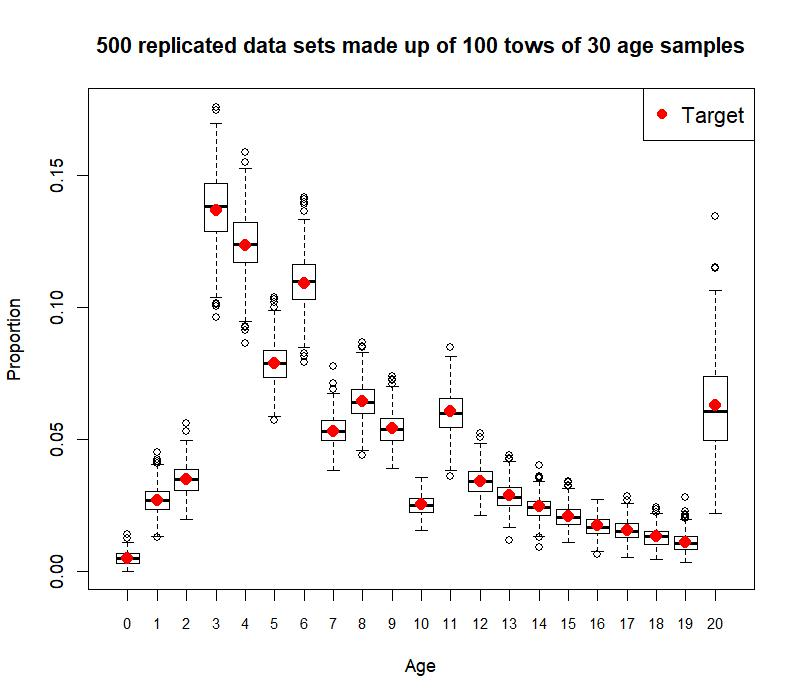
\includegraphics[scale=0.5]{Figures/MH_samples.jpeg}
	\caption{Boxplots of simulated age frequency using the algorithm described in the methods, with $n_a = 30$ (number of otoliths per cluster), $n_c = 100$ (number of clusters) and $\sigma_c = 2.5$, showing that on average they generate unbiased proportions at age.}
	\label{fig:simulated_MH_data}
\end{figure}

\begin{figure}[!h]
	\centering
	\subfloat[]{
	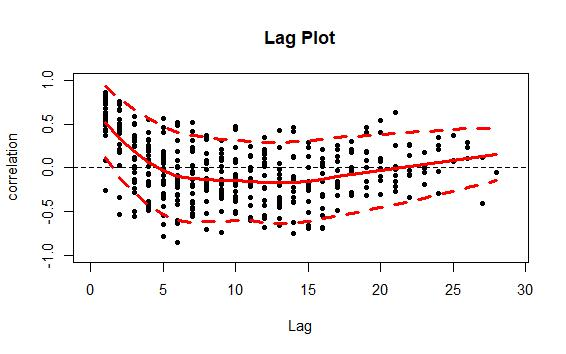
\includegraphics[scale=0.6]{Figures/cluster_residuals_post_dataweighting.png}}
	\qquad
	\subfloat[]{
	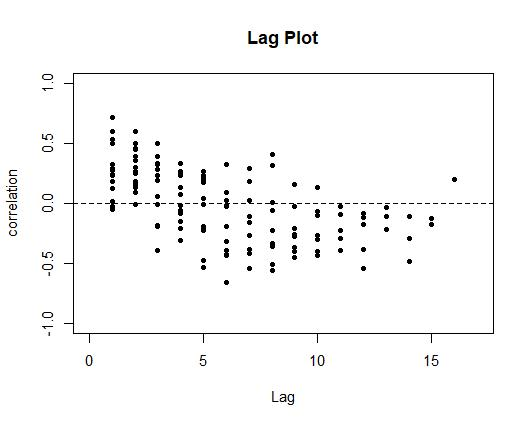
\includegraphics[scale=0.6]{Figures/chatTANage_resid_corr.jpg}}
	\caption{Top panel (a) are, Pearson residuals from a stock assessment assuming a multinomial distribution, with data simulated from the IBM with this cluster algorithm. The bottom panel (b)are Pearson residuals, from the HAK 3\&4 stock assessment from the Chatham Rise Age composition data set.}
	\label{fig:ResidsConsistent}
\end{figure}

\pagebreak
\subsubsection{Age frequency from Mortality Event Biomass process with clustering}\label{subsubsec:MortalityEventBiomasssubsamlecluster}\index{Observations!Age frequency from Mortality Event Biomass With Clustering}

In this observation, you specify the number of clusters which can be thought of as hauls you want to sample from a fishing event (specific fishery and time), as well as some attributes of clusters i.e.  \subcommand{average\_cluster\_weight} in tonnes average weight of haul to sample, the cv \subcommand{cluster\_cv} which describes the variance around the mean weight of hauls to sample from (distribution assumed is log normal). Within each cluster you can specify, how many otoliths will be sampled from each haul, and how correlated the ages will be within a haul, this is defined by the \subcommand{cluster\_sigma}. As this parameter goes to zero the hauls are highly homogeneous, compared to a large value, where the ages become uncorrelated. You can ask for the observation to be normalised as proportions (\subcommand{composition\_type proportions} ) or as numbers. 



The other neat thing regarding this observation class, is you can weight each haul, 




The algorithm

\begin{itemize}
	\item Iterate over each stratum, calculating weight in each stratum, and associated cells with their weights
	\item for each stratum
	\subitem iterate over all cells within each strata 
	\subitem with in each cell
	\subsubitem randomly select a cluster/haul, number of hauls per cell are weighted by how much biomass was in the cell compared to all cells within strata
	\subsubitem Randomly select a cluster size (weight based quantity)
	\subsubitem Calculate that to abundance using a simple mean weight per agent in the cell.
	\subsubitem Randomly select on agent in available in the current cell, this is the starting agent, and all other agents in the cluster are conditional on this first agent (thus creating a school effect)
	\subsubitem We implement a Metropolis Hastings algorithm (steps~\ref{list:MH_algorithm}) to select the number agents that the user desires for this cluster.
	\subsubitem Can apply ageing error at this point
	\subsubitem weight each aged fish's contribution by the weight of the cluster e.g. an aged fish from a cluster of 100 tonnes will have more 'weight' than an aged fish from a cluster of 1 tonne.
\end{itemize}
%

\begin{enumerate}\label{list:MH_algorithm}
	\item Randomly select an individual $x_0$ from the population (all individuals have equal probability of capture)
	
	\item generate a proposal individual from  $x'_i \sim \mathcal{N}(x_{i-1}, \sigma_c^2)$
	
	\item calculate the acceptance ratio $\alpha = \frac{\pi(x'_i)}{\pi(x_{i-1})}$
	
	\item accept if $u \leq \alpha$ $x_i = x'_i$ or reject if $u > \alpha$ $x_i = x_{i-1}$
	
	\item repeat steps 2-4 until an adequate sample size is reached denoted by \(n_a\).
	
	\item repeat steps 1-5 to generate multiple clusters \(n_c\)
\end{enumerate}


\subsubsection{Tag-recaptures by length}\label{subsubsec:tag_recap_by_length}\index{Observations!Tag-recaptures by length}


\subsubsection{Tag-recaptures by age}\label{subsubsec:tag_recap_by_age}\index{Observations!Tag-recaptures by age}


\subsection{\I{Ageing error}}\label{subsec:ageing_error}
\IBM\ can apply ageing error to an expected age frequency generated by the model. The ageing error is applied as a misclassification matrix, which has the effect of 'smearing' the expected age frequencies. This is mimicking the error involved in identifying the age of individuals. For example fish species are aged by reading the ear bones (otoliths) which can be quite difficult depending on the species. These are used in generating age based observations. 

Ageing error is optional, and if it is used, it may be omitted for any individual time series. Different ageing error models may be applied for different observation commands. See Section \ref{sec:ageingerrorreport} for reporting the misclassification matrix at the end of model run.

The ageing error models implemented are,
\begin{enumerate}
	\item{None}: The default model is to apply no ageing error.
	\item{Off by one}: Proportion $p_1$ of individuals of each age $a$ are misclassified as age $a-1$ and proportion $p_2$ are misclassified as age $a+1$. Individuals of age $a < k$ are not misclassified. If there is no plus group in the population model, then proportion $p_2$ of the oldest age class will 'fall off the edge' and disappear. 
	\item{Normal}: Individuals of age $a$ are classified as ages which are normally distributed with mean $a$ and constant c.v. $c$. As above, if there is no plus group in the population model, some individuals of the older age classes may disappear. If $c$ is high enough, some of the younger age classes may 'fall off the other edge'. Individuals of age $a < k$ are not misclassified.
\end{enumerate}

Note that the expected and simulated observations reported by \IBM\ for observations with ageing error will have had the ageing error applied. 

